\documentclass{article}

\usepackage{amsmath}
\usepackage{amssymb}
\usepackage[margin=1in]{geometry}
\usepackage{enumitem}
\usepackage{hyperref}
\usepackage{tikz}
\usetikzlibrary{arrows,automata}

\begin{document}
	\noindent\begin{large}\textbf{Topic: Searching Problem Formulation}\end{large}
	
	\begin{enumerate}
		\item \begin{enumerate}
			\item Assuming the grid is $n \times m$, we have $4 \times n \times m$ unique states in our space.
			\item I don't see how this affects the upper-bound for our state space size. If we assume each corridor is one square in length and has 4 directions to choose from, it is the same size. We could say that we don't want to turn around, which would reduce it to $3 \times n \times m$. I am probably misinterpreting this problem.
		\end{enumerate}
		\item To reduce the number of states, I only included valid steps. The correct path is clearly shown. \begin{enumerate}
			\item 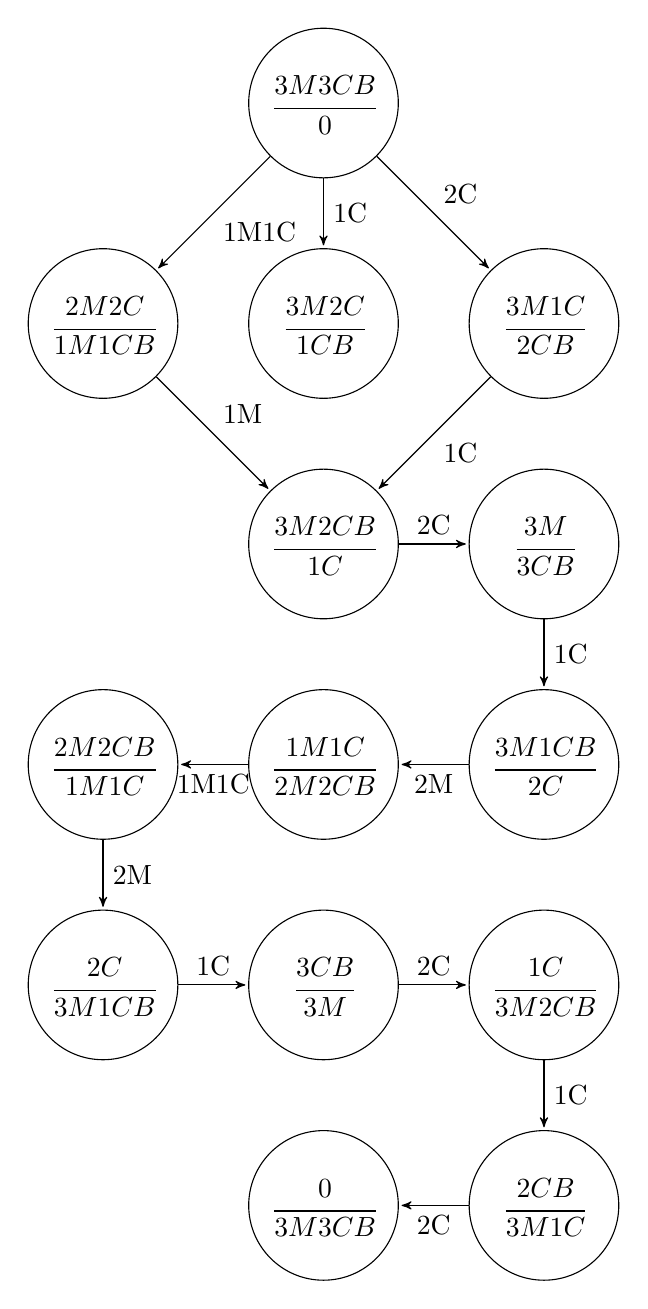
\begin{tikzpicture}[baseline=(A.north),->, >=stealth',shorten >=1pt, auto, node distance=2.8cm]
				\tikzstyle{every state} = [minimum size=1.9cm];
				\node[state] (A) {$\cfrac{3M3CB}{0}$};
				
				\node[state] (B) [below of=A] {$\cfrac{3M2C}{1CB}$};
				\node[state] (C) [left of=B] {$\cfrac{2M2C}{1M1CB}$};
				\node[state] (D) [right of=B] {$\cfrac{3M1C}{2CB}$};
				
				\node[state] (E) [below of=B] {$\cfrac{3M2CB}{1C}$};
				
				\node[state] (F) [right of=E] {$\cfrac{3M}{3CB}$};
				
				\node[state] (G) [below of=F] {$\cfrac{3M1CB}{2C}$};
				
				\node[state] (H) [left of=G] {$\cfrac{1M1C}{2M2CB}$};
				
				\node[state] (I) [left of=H] {$\cfrac{2M2CB}{1M1C}$};
				
				\node[state] (J) [below of=I] {$\cfrac{2C}{3M1CB}$};
				
				\node[state] (K) [right of=J] {$\cfrac{3CB}{3M}$};
				
				\node[state] (L) [right of=K] {$\cfrac{1C}{3M2CB}$};
				
				\node[state] (M) [below of=L] {$\cfrac{2CB}{3M1C}$};
				
				\node[state] (N) [left of=M] {$\cfrac{0}{3M3CB}$};
				
				\path (A) edge node {1C} (B)
						  edge node {1M1C} (C)
						  edge node {2C} (D)
					  (C) edge node {1M} (E)
					  (D) edge node {1C} (E)
					  (E) edge node {2C} (F)
					  (F) edge node {1C} (G)
					  (G) edge node {2M} (H)
					  (H) edge node {1M1C} (I)
					  (I) edge node {2M} (J)
					  (J) edge node {1C} (K)
					  (K) edge node {2C} (L)
					  (L) edge node {1C} (M)
					  (M) edge node {2C} (N);
			\end{tikzpicture}
		\end{enumerate}
	\end{enumerate}
\end{document}